\documentclass[a4paper,twoside,12pt,chapterprefix=false,listof=flat]{scrartcl}
\usepackage{lmodern}
\usepackage{amssymb,amsmath}
\usepackage{ifxetex,ifluatex}
\usepackage{fixltx2e} % provides \textsubscript
\ifnum 0\ifxetex 1\fi\ifluatex 1\fi=0 % if pdftex
  \usepackage[T1]{fontenc}
  \usepackage[utf8]{inputenc}
\else % if luatex or xelatex
  \ifxetex
    \usepackage{mathspec}
  \else
    \usepackage{fontspec}
  \fi
  \defaultfontfeatures{Ligatures=TeX,Scale=MatchLowercase}
\fi
% use upquote if available, for straight quotes in verbatim environments
\IfFileExists{upquote.sty}{\usepackage{upquote}}{}
% use microtype if available
\IfFileExists{microtype.sty}{%
\usepackage[]{microtype}
\UseMicrotypeSet[protrusion]{basicmath} % disable protrusion for tt fonts
}{}
\PassOptionsToPackage{hyphens}{url} % url is loaded by hyperref
\usepackage[unicode=true]{hyperref}
\hypersetup{
            pdftitle={DPs Syntax in acquisition},
            pdfauthor={Marco Petolicchio},
            pdfborder={0 0 0},
            breaklinks=true}
\urlstyle{same}  % don't use monospace font for urls
\usepackage{natbib}
\bibliographystyle{apa}
\usepackage{longtable,booktabs}
% Fix footnotes in tables (requires footnote package)
\IfFileExists{footnote.sty}{\usepackage{footnote}\makesavenoteenv{long table}}{}
\usepackage{graphicx,grffile}
\makeatletter
\def\maxwidth{\ifdim\Gin@nat@width>\linewidth\linewidth\else\Gin@nat@width\fi}
\def\maxheight{\ifdim\Gin@nat@height>\textheight\textheight\else\Gin@nat@height\fi}
\makeatother
% Scale images if necessary, so that they will not overflow the page
% margins by default, and it is still possible to overwrite the defaults
% using explicit options in \includegraphics[width, height, ...]{}
\setkeys{Gin}{width=\maxwidth,height=\maxheight,keepaspectratio}
\IfFileExists{parskip.sty}{%
\usepackage{parskip}
}{% else
\setlength{\parindent}{0pt}
\setlength{\parskip}{6pt plus 2pt minus 1pt}
}
\setlength{\emergencystretch}{3em}  % prevent overfull lines
\providecommand{\tightlist}{%
  \setlength{\itemsep}{0pt}\setlength{\parskip}{0pt}}
\setcounter{secnumdepth}{5}
% Redefines (sub)paragraphs to behave more like sections
\ifx\paragraph\undefined\else
\let\oldparagraph\paragraph
\renewcommand{\paragraph}[1]{\oldparagraph{#1}\mbox{}}
\fi
\ifx\subparagraph\undefined\else
\let\oldsubparagraph\subparagraph
\renewcommand{\subparagraph}[1]{\oldsubparagraph{#1}\mbox{}}
\fi

% set default figure placement to htbp
\makeatletter
\def\fps@figure{htbp}
\makeatother

%\usepackage[a4paper,left=4.5cm, top=3.5cm, bottom=3.5cm, right=4.5cm, heightrounded, headsep=2em, footskip=11mm, vmarginratio=1:1]{geometry}
\usepackage[a4paper,margin=4cm,  heightrounded, headsep=2em, footskip=11mm, vmarginratio=1:1]{geometry}
\makeatletter
\DeclareOldFontCommand{\rm}{\normalfont\rmfamily}{\mathrm}
\DeclareOldFontCommand{\sf}{\normalfont\sffamily}{\mathsf}
\DeclareOldFontCommand{\tt}{\normalfont\ttfamily}{\mathtt}
\DeclareOldFontCommand{\bf}{\normalfont\bfseries}{\mathbf}
\DeclareOldFontCommand{\it}{\normalfont\itshape}{\mathit}
\DeclareOldFontCommand{\sl}{\normalfont\slshape}{\@nomath\sl}
\DeclareOldFontCommand{\sc}{\normalfont\scshape}{\@nomath\sc}
\makeatother




\usepackage{fontspec}

\usepackage{ifluatex}

\usepackage{microtype}



\setmainfont[Numbers=Lowercase]{IBMPlexSerif}
\setsansfont[Numbers=Lowercase]{IBMPlexSans}
\setmonofont[Numbers=Lowercase, Scale=.8]{IBMPlexMono}


\usepackage[english]{babel}





\usepackage[all]{nowidow}






\usepackage[usenames, dvipsnames]{xcolor}
\definecolor{upol-dGrey}{rgb}{0.36470588235,0.36862745098,0.37647058823}
\definecolor{upol-lGrey}{rgb}{0.8,0.8,0.8}
\definecolor{upol-brandBlue}{rgb}{0,0.43529411764,0.67843137254}


\usepackage{xcolor}
\usepackage{graphicx}
\definecolor{titlepagecolor}{cmyk}{1,.38,0,.15} %C100 M38 Y0 K15
\definecolor{namecolor}{cmyk}{0, 0, 0, .0980} 
\usepackage{textcase}


\usepackage{setspace}

\makeatletter\let\Title\@title\makeatother
%\makeatletter\let\Author\@author\makeatother



\usepackage{sectsty}
\allsectionsfont{\color{upol-dGrey}\sffamily}
\chapterfont{\color{upol-dGrey}\raggedleft\thispagestyle{empty}}





\usepackage{floatrow}
\floatsetup[table]{font=sf}
\floatsetup[figure]{font=sf}
\floatsetup[tikzpicture]{font=sf}

\usepackage[font={color=upol-dGrey}, labelfont={color=upol-dGrey}]{caption}



\makeatletter
\def\verbatim@font{\linespread{1}\footnotesize\ttfamily}
\makeatother



\makeatletter
\renewenvironment{figure}[1][\fps@figure]{
  \edef\@tempa{\noexpand\@float{figure}[#1]} 
  \@tempa
  \sffamily
}{
  \end@float
}
\renewenvironment{table}[1][\fps@table]{
  \edef\@tempa{\noexpand\@float{table}[#1]} 
  \@tempa
  \sffamily
  \footnotesize
}{
  \end@float
}
\makeatother

\usepackage{tabularx,tabu}
\usepackage{amsfonts}
\usepackage{booktabs}
\usepackage{siunitx}
\usepackage{fancyhdr}

\usepackage{lipsum, kantlipsum} % just for testing

\pagestyle{fancy}
\fancyhf{}
\fancyhead[LE,RO]{\thepage}
%\fancyhead[RE]{\footnotesize\nouppercase{\leftmark}}
\fancyhead[RE]{\footnotesize\nouppercase{M. Petolicchio, \textit{DPs Syntax in acquisition}}}
\fancyhead[LO]{\footnotesize\nouppercase{\rightmark}}
\setlength{\headheight}{14.5pt} % as requested by fan
\renewcommand{\headrulewidth}{0pt}

\renewcommand{\chaptermark}[1]{\markboth{\thechapter \ . \  #1}{}}
\renewcommand{\sectionmark}[1]{\markright{\thesection \ \ #1}{}}





%\setcounter{secnumdepth}{5}
%\setsecnumdepth{subsubsection}
%\maxtocdepth{subsubsection}


\setlength{\skip\footins}{3em}
\renewcommand\footnoterule{{\hrule height 0pt}} % a long blue line



\usepackage{colortbl}
\arrayrulecolor{gray}







\usepackage{booktabs}

\usepackage{pdfpages}






%Options: Sonny, Lenny, Glenn, Conny, Rejne, Bjarne, Bjornstrup
\usepackage[Bjornstrup]{fncychap}
%\renewcommand{\CNoV}{\raggedleft\sffamily\selectfont\HUGE}
  \ChNumVar{\Huge\sffamily\selectfont}
\renewcommand{\DOCH}{%
   \settowidth{\py}{\CNoV\thechapter}
  \addtolength{\py}{1em}      % Amount of space by which the
%                                % number is shifted right
   \fboxsep=0pt%
   \colorbox[gray]{.85}{\rule{0pt}{50pt}\parbox[b]{\textwidth}{\hfill}}%
   \kern-\py\raise20pt%
   \hbox{\color{gray}\CNoV\thechapter}\\%
}

\makeatletter
\renewcommand*{\@makechapterhead}[1]{%
  \vspace*{0\p@}%
  {\parindent \z@ \raggedright \normalfont
    \ifnum \c@secnumdepth >\m@ne
      \if@mainmatter%%%%% Fix for frontmatter, mainmatter, and backmatter 040920
        \DOCH
      \fi
    \fi
    \interlinepenalty\@M
    \if@mainmatter%%%%% Fix for frontmatter, mainmatter, and backmatter 060424
      \DOTI{#1}%
    \else%
      \DOTIS{#1}%
    \fi
  }}
% For the case \chapter*:
\renewcommand*{\@makeschapterhead}[1]{%
  \vspace*{10\p@}%
  {\parindent \z@ \raggedright
    \normalfont
    \interlinepenalty\@M
    \DOTIS{#1}
    \vskip 0\p@
  }}
\makeatother





\usepackage{tikz,tikz-qtree}


\tikzstyle{every picture}+=[font=\sffamily]

\usepackage{listings}
\lstset{ %Formatting for code in appendix
	backgroundcolor = \color{gray},
	language=Python,
	basicstyle=\singlespacing\footnotesize\ttfamily\color{white},
	numbers=left,
	stepnumber=1,
	showstringspaces=true,
	tabsize=2,
	breaklines=true,
	breakatwhitespace=false,
	xleftmargin=3em,framexleftmargin=3em, numberstyle=\ttfamily,
}

\usepackage{datetime}

%\let\oldmaketitle\maketitle
%\AtBeginDocument{\let\maketitle\relax}




\usepackage{catchfilebetweentags}

\usepackage[autostyle]{csquotes}  
\usepackage{enumerate}


\makeatletter
\newcommand\HUGE{\@setfontsize\Huge{36}{48}} 
\makeatother

\usepackage{tikz}
\usepackage{pgfplots}


\usepackage{gb4e,cgloss}
\noautomath
\let\eachwordone=\itshape


\usepackage{amsthm}

\theoremstyle{plain} % default
\newtheorem{theorem}{Theorem}[section]
\newtheorem{lemma}[theorem]{Lemma}
\newtheorem{proposition}[theorem]{Proposition}
\newtheorem*{corollary}{Corollary}

\theoremstyle{definition}
\newtheorem{definition}{Definition}[section]
\newtheorem{conjecture}{Conjecture}[section]
\newtheorem{example}{Example}[section]
\newtheorem{postulate}{Postulate}[section]
\newtheorem{problem}{Problem}[section]

\theoremstyle{remark}
\newtheorem*{remark}{Remark}
\newtheorem*{note}{Note}
\newtheorem{case}{Case}

\title{DPs Syntax in acquisition}
\providecommand{\subtitle}[1]{}
\subtitle{A case study on Italian L2 by Czech ad Slovak learners}
\author{Marco Petolicchio}
\date{}

\begin{document}
\maketitle
\begin{abstract}
Czech and Slovak are languages which don't exhibit a manifest position
for the Articles in the Determiner Phrase. The aim of this paper is to
show how this structure is accessed during the learning of Italian, a
language which presents the articles as for the standard behavior for
nouns.\par \textbf{Keywords:} Determiner Phrase, Italian L2, Second
Language Acquisition, Syntax
\end{abstract}

{
\setcounter{tocdepth}{2}
\tableofcontents
}
\clearpage

\section{Introduction}\label{introduction}

Czech (\texttt{ces}) and Slovak (\texttt{slk}) are languages of the
Slavic branch in the Indo-european family. Alongside a certain
morphological complexity in noun declension systems, these languages
--except for Bulgarian (\ref{exm:dpBul}) and Macedonian
\citep{wals-37}-- don't show an overt realization of the Determiner
position inside the noun phrase (\ref{exm:dpNo}) \citep{harkins1953}.
Conversly, Italian (\texttt{ita}) and the other romance languages
explicit that position as a default behaviour, usually with a free
morpheme preceding the noun (\ref{exm:dpPre}) or by cliticization of the
definite article (\ref{exm:dpRon}):

\begin{enumerate}
\def\labelenumi{(\arabic{enumi})}
\tightlist
\item
  Articleless \label{exm:dpNo}

  \begin{enumerate}
  \def\labelenumii{\alph{enumii}.}
  \tightlist
  \item
    \texttt{ces} \citep[ 14]{veselovska2014}\\
    \gll    Chlapec/Marie/Ona/každý miluje ryby/ \{své rodiče\}.\\
    Boy/Marie/She/Everyone Love.3sg Fish/ \{POSS parent\}\\
    \glt    \enquote{SUBJ loves {[}the{]} fish/ his parents}
  \item
    \texttt{slk} \citep[ 113]{krizomkrazomA1}\\
    \gll    Večer čítam knihy, píšem referatý\ldots{}\\
    Evening Read.1SG Book.PL Write.1SG Paper.PL\\
    \glt    \enquote{In the evening I read {[}the{]} books, I write
    (school) papers \ldots{}}
  \end{enumerate}
\item
  Proclitic \label{exm:dpPre}

  \begin{enumerate}
  \def\labelenumii{\alph{enumii}.}
  \tightlist
  \item
    \texttt{ita} \citep[ 60]{bianco2017}\\
    \gll    Il terremoto ha distrutto la città.\\
    ART.DEF Earthquake AUX.3sg Destroy.PTCP.PST ART.DEF City\\
    \glt    \enquote{The earthquake destroyed the city}
  \item
    \texttt{fro} \citep[ 3261]{dedole2008}\\
    \gll    La dame estoit devant la sale.\\
    ART.DEF Girl Be.3sg ADV ART.DEF Room\\
    \glt    \enquote{The \emph{dame} was in front to the room}
  \end{enumerate}
\item
  Enclitic

  \begin{enumerate}
  \def\labelenumii{\alph{enumii}.}
  \tightlist
  \item
    \texttt{ron} \citep[ 45]{cojocaru2003} \label{exm:dpRon}\\
    \gll    Prieten=ul meu este aici.\\
    Friend=ART.DEF POSS Be.PRES.3sg Here\\
    \glt    \enquote{My friend is here}
  \item
    \texttt{bul} \citep[ 37]{leafgren2011} \label{exm:dpBul}\\
    \gll    Къде е книга=та ми?\\
    Where Be.3SG Book=ART.DEF POSS.1SG\\
    \glt    \enquote{Where is my book?}
  \end{enumerate}
\end{enumerate}

The general idea of this paper is to address the question of how
linguistic structures which are not overtly marked in L1 can be accessed
during the acquisition of a target language that show them. While doing
this can be either both purely speculative as grounded on actual data, I
will show how the usage of a target collection of linguistic corpora can
be useful to test the main hypotheses into narrower facts. The language
under observation are indeed a few: on one side \texttt{ces} and
\texttt{slk} as native languages--with no overt position for the
articles--on the other \texttt{ita} as target language.

The section \ref{sec:theoryBg} provides a theoretical discussion on the
top of different theories inside the Generative framework
\citep{chomsky1995} on the status of DP and NP. The section
\ref{sec:caseStudy} is twofold: firstly I present the methods used into
the current analysis in terms of \emph{reproducibility} of the research,
the policies of data-collection and an analysis of the expected results;
while the second subsection is built upon a case study made off to test
some hypotheses about the categorial differences of DPs during the
acquisition of \texttt{ita} by \texttt{ces} and \texttt{slk} native
speakers involved in the test. A summary conclusion (Section
\ref{sec:concl}) closes the paper.

\section{Theoretical background}\label{sec:theoryBg}

One of the main area of research in Generative studies on Second
Language Acquisition (\texttt{GenSLA}) regards the investigation about
how the linguistic structures can be accessed in L2 and how the
transitional stages of acquisition work into the learning continuum
\citep{rothmanslabakova2017}.

\subsection{The position of DP and NP}\label{the-position-of-dp-and-np}

There are striking differencies amongst languages that display an overt
D position and those that do not do it in respect to the syntactic
behaviour of NP, as such as Left Branch Extraction allowing, scrambling
or adjective extraction. Those are properties are summarized in the
table below \citep[in][ from \citet{boskovic2009}]{salzmann2018}:

\begin{longtable}[]{@{}lll@{}}
\caption{Syntactic differencies amongst overt/covert D
languages}\tabularnewline
\toprule
& overt D & covert D\tabularnewline
\midrule
\endfirsthead
\toprule
& overt D & covert D\tabularnewline
\midrule
\endhead
allow adj extraction from NP & no & yes\tabularnewline
allow LBE & no & yes\tabularnewline
allow Neg-raising & yes & no\tabularnewline
allow scrambling & no & yes\tabularnewline
allow the majority superlative reading & yes & no\tabularnewline
allow trans. nominals with 2 non-lex. genitives & yes &
no\tabularnewline
can be polysynthetic & no & yes\tabularnewline
island sensitivity in head-internal relatives & no & yes\tabularnewline
superiority effects in wh-mvt & yes & no\tabularnewline
\bottomrule
\end{longtable}

Since the seminal work of \citep{abney1987} there have been established
two hypothesis to represent this structure: (i) NP-over-DP, for which
the DP is at the edge of NP as specifier; (ii) DP-over-NP, where the DP
dominates the NP:

\begin{figure}

{\centering 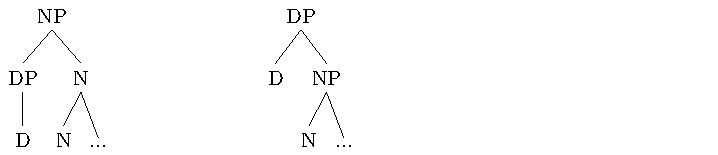
\includegraphics[width=1\linewidth]{_main_files/figure-latex/tree1-1} 

}

\caption{Structural comparison between NP-over-DP and DP-over-NP Hypotheses}\label{fig:tree1}
\end{figure}

\subsubsection{Implications for the DP-Hypothesis in
Italian}\label{implications-for-the-dp-hypothesis-in-italian}

Symmetries amongst the DP/NP phrase and the whole sentence are often
referenced in terms of structure building and phase-related properties
\citep{chomsky2013, chomsky2015}.

\subsubsection{Implications for the DP-Hypothesis in
Czech}\label{implications-for-the-dp-hypothesis-in-czech}

\subsection{The role and the study on
interlanguage}\label{the-role-and-the-study-on-interlanguage}

\section{Case Study}\label{sec:caseStudy}

\subsection{Retrieve the linguistic
data}\label{retrieve-the-linguistic-data}

This analysis relies on 3 corpora of Italian L2, subsetted for the
current purposes of having Czech and Slovak L1.

\begin{table}

\caption{\label{tab:unnamed-chunk-5}Amount of data in the collection}
\centering
\begin{tabu} to \linewidth {>{\raggedright}X>{\raggedright}X>{\raggedright}X>{\raggedright}X>{\raggedright}X}
\toprule
\multicolumn{1}{c}{ } & \multicolumn{2}{c}{Texts} & \multicolumn{2}{c}{Tokens} \\
\cmidrule(l{2pt}r{2pt}){2-3} \cmidrule(l{2pt}r{2pt}){4-5}
  & ces & slk & ces & slk\\
\midrule
Czech-IT & 212 & 74 & 11129 & 4440\\
Merlin & 1 & 0 & 256 & 0\\
Valico & 107 & 17 & 16250 & 3316\\
\bottomrule
\end{tabu}
\end{table}

\begin{figure}
\centering
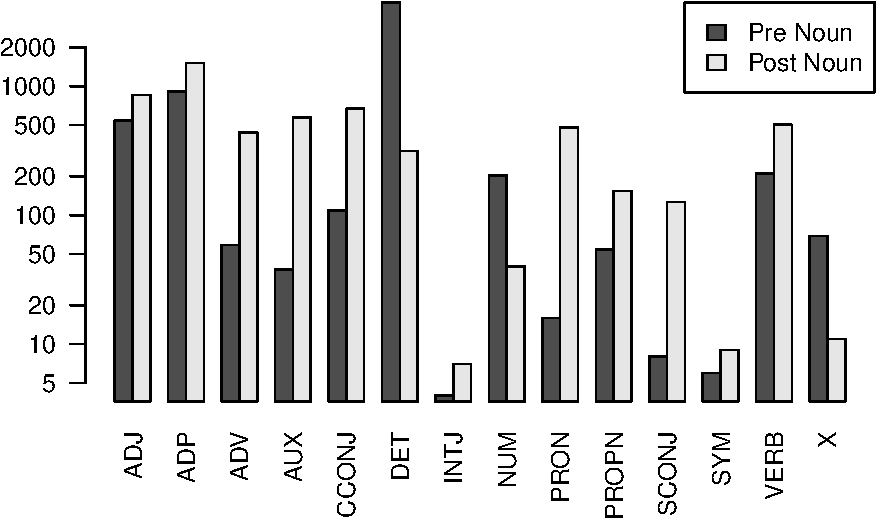
\includegraphics{_main_files/figure-latex/graphNoun-1.pdf}
\caption{\label{fig:graphNoun}Bi-grams distribution of elements near Nouns}
\end{figure}

\subsection{Perform a test}\label{perform-a-test}

Provide 10 noun phrases with different referential structure in terms of
animateness with a neutralized article. The students are invited to
write full sentences for each one.

Goals:

\begin{itemize}
\tightlist
\item
  Test the syntactic distribution of phrases (SUBJ vs OBJ)
\item
  Test the distribution of DETs ({[}+def{]}, {[}-def{]}, Ø)
\end{itemize}

\section{Conclusion}\label{sec:concl}

\section*{Financial coverage}\label{financial-coverage}
\addcontentsline{toc}{section}{Financial coverage}

This work was partially supported by the funding grant XXX.

\section*{Abbreviations}\label{abbreviations}
\addcontentsline{toc}{section}{Abbreviations}

Languages are indicated by the abbreviations provided in the ISO 639-3
format \citep{iso639-3}. Morphological glosses styles adher to the
widespreadly recognized \emph{Leipzig Glossing Rules}
\citep{leipzigGlossingRules}, while other abbreviations respect
\citep{boeckxListOfAbbreviations}.

\bibliography{bibliography.bib}

\end{document}
